% Paper for the IWINAC 2013
% created by LP
% December 15, 2012
%
\documentclass[runningheads,a4paper]{llncs}

\usepackage{amssymb}
\usepackage{xfrac}
\setcounter{tocdepth}{3}
\usepackage{graphicx}

\usepackage[utf8]{inputenc}

\usepackage{url}
\urldef{\mailsa}\path|lporrasdiaz@gmail.com|
\newcommand{\keywords}[1]{\par\addvspace\baselineskip
\noindent\keywordname\enspace\ignorespaces#1}


\newcommand{\nats}{\mathbb{N}}
\newcommand{\connex}{\mathit{connex}}

\usepackage{xcolor}
\usepackage{todonotes}

\begin{document}

  %\mainmatter  % start of the contributions

  \title{Bursting P systems: A proposal for modelling and simulation of genetic regulatory networks}

  \titlerunning{Bursting P systems} % abbreviated title (for running head)
%                                     also used for the TOC unless
%                                     \toctitle is used

  \author{Luis Porras D\'iaz}
 
  \authorrunning{Luis Porras D\'iaz}   % abbreviated author list (for running head)
 

  \institute{
    Departamento de Inteligencia Artificial, Facultad de Informática,\\
    Universidad Politécnica de Madrid, 28660 Boadilla del Monte, Madrid, Spain\\
    \mailsa\\
  }
  %%%% modified list of authors for the TOC (add the affiliations)
  \tocauthor{
  Luis Porras D\'iaz(UPM)
  }

  \maketitle              % typeset the title of the contribution

  \begin{abstract}
    This paper introduces \emph{bursting P systems} (BP systems) as a new formal
    framework for specifying and simulating computational models of genetic
    regulatory networks. BP systems are based on spiking neural P systems in an
    attempt to capture the spikiness of signal transmission in gene networks. One
    singular feature of BP systems is that they include several types of spikes
    since different proteins can be used as signal transmitters within the network.
    Additionally, probability functions are used instead of regular expressions to
    decide whether or not a rule should be triggered depending on the number of
    transcription factors. A model of a synthetic oscillatory gene network, the
    \textit{repressilator}, is used as case study.
  \end{abstract}
 
  \section{Introduction}
  \color{gray}
  \todo[inline]{ Area is, understand genetic circuits}
  The big challenge in biology to understand how the expression of genes result in 
  particular behaviours of a cell. 
  In recent years the fields of synthetic and systems biology are bringing new
  tools and advanced techniques to help understand and control the expression of genes. 
  As we learn more about genetic circuits from theoretical and laboratory studies 
  we start to understand more about how gene networks work. 
  A recent discovery is the spikiness of gene expression. 

  \todo[inline]{List of models and explain their good and bad points}
  Some models that are currently used to successfully model genetic circuits are 
    petri nets
    ODEs 
    Frans system. 

  \todo[inline]{Maybe some vague alusion to Uri Alon's metaphore?}
  Inspired by this we spikiness and the comparison of e. coli genetic networks 
  to a brain we have a model that tries to capture the spikes of genetic expression.

  \todo[inline]{Why we made this model}
  The point of this model is to attempt to build up a heirarcical frame work of 
    gene expression. 
  
  Our model has the following characteristics, 
    Compartmentalised 
      Reactants are not well diffused throughout a cell. 
      Reactants are often clustered in specific areas and Eucaryotes and bacteria 
      have vessicles to contain reactants to speed chemical reactions. 
      Frans Model also has the compartmentalised characteristic. 
    This allows us to nest these structures and study multi compartmental expression 
      that might yeild interesteing results for tissue like systems and allow us 
      to study embryo formation.

  Our model aims at mathematical and analysis, we are less interested in quantitatively 
  simulating these systems as we are in studying the dynamics. 

  For this reason we use the framework of membrane systems to implement our model.
  This allows us to build on the substantial body of theoretical research 
  built up for various models. 
  \color{black}

  \todo[inline]{Membranes history, reduce to 5 lines}
  Membrane computing~\cite{Paun2000} is a field of natural computing. It was
  originally devised as a new computational model inspired by cell structure and
  some biochemical processes that take place inside cells. Properly formalized,
  these processes can be interpreted as computational operations. A membrane
  computing system, also known as a \emph{P system}, is built from a hierarchy of
  compartments (membranes). Rewrite rules, called \emph{evolution rules}, are
  executed in parallel on multi-sets of symbols in each compartment. Each
  membrane is in contact with the adjoining membranes in the hierarchy, whereby
  one or more symbols from one membrane can transfer to the adjoining membranes
  as a result of the execution of a rule. A P system with these elements is a
  Turing-complete distributed and parallel processing system that efficiently
  solves problems of high algorithmic complexity.

  Other variants based on this initial idea of P system were later proposed,
  such as \emph{tissue P systems}~\cite{MartinVide2003}. In tissue P systems,
  the model compartments are equivalent not to cell membranes but to cells
  integrated into tissue. Communication channels can be established between
  cells in the shape of a graph, rather than a tree as in the original P
  systems. Similarly, neural tissue is the source of \emph{spiking neural P
    systems} (SNPS)~\cite{Ionescu2006}. The aim behind these systems is to
  build the features of nerve impulses into P systems. To do this, SNPS build
  graph-like structures. The nodes of these graphs are the neurons and the
  edges are the synapses that pass the copies of a single object, representing
  a nerve impulse (\emph{spike}). In these systems, the internal state of each
  neuron is associated with the number of spikes that it contains, and they
  also use time as another computational tool. This way, they are capable of
  performing computational operations based on information encoded in the spike
  emission/reception frequency.

  These three basic types of P systems have spawned a huge number of articles
  studying the potential of these models for language or number set generation
  and acceptance, as well as NP-complete problem
  solving~\cite{Paun2001}~\cite{Leporati2009}. Additionally, many variants have
  been proposed adding or removing model elements to examine their
  computational capacity and
  efficiency~\cite{Cavaliere2004}~\cite{Alhazov2005}~\cite{Cavaliere2008}~\cite{Cavaliere2009}.
  But, beyond their use as simple abstract computing devices, new lines of
  research have focused on searching for a practical application of P systems
  for modelling biological processes taking place at cellular level. Thus, for
  example,~\cite{Paun2006} propose a P system variant for modelling biochemical
  signal propagation cascades involved in epidermal growth factor reception. In
  this model, the system evolution is driven by the \emph{deterministic waiting
    time algorithm} that \emph{decides} the order in which the rules are
  executed based on their speed of reaction mediated by the number of reactant
  molecules. As opposed to this deterministic strategy,~\cite{Bernardini2006}
  propose a stochastic alternative based on the Gillespie
  algorithm~\cite{Gillespie1977} to model a \emph{quorum sensing system} in
  \emph{Vibrio fischeri} bacteria. The two strategies are reviewed and compared
  in~\cite{PerezJimenez2006}. ~\cite{RomCamp2007} present several cellular
  processes, such as protein transformation, degradation,
  formation/dissociation and gene expression, modelled by P systems.
  Again~\cite{Gheorghe2010} examine two different evolution strategies, a
  stochastic strategy used in stochastic P systems based on the Gillespie
  algorithm~\cite{Gillespie1977} and a deterministic strategy used in metabolic
  P systems, illustrated by examples of the \emph{repressilator} and the
  \emph{mitotic oscillator}. Additionally,~\cite{Busi2006}
  and~\cite{RomCamp2008} also propose other P system-based gene expression
  control models.~\cite{Busi2006} apply their model to the construction of a
  genetic RAM memory, whereas~\cite{RomCamp2008} build a model of the LAC
  operon.

  However, none of the above models account for the spikiness of gene
  regulatory networks: bursts of messenger RNA (mRNA) form during gene
  transcription~\cite{Golding2005,Chubb2006,Raj2006}. One
  explanation for this phenomenon is that these bursts occur at the exact same
  time as a transcription factor molecule binds to the gene promoter region.
  Likewise, a bound molecule can also separate, meaning that the gene in
  question will momentarily stop transcribing mRNA. In the meantime, another
  molecule may take the place of the separated molecule, triggering another
  burst. The likelihood of separated molecules being replaced by others depends
  on how much transcription factor is present in the cell: binding and,
  therefore, the emission of another burst is more likely the more
  transcription factor there is. Thus, gene transcription can be viewed as a
  succession of bursts whose frequency is modulated by the concentration of
  transcription factors.

  With a view to building a formal model, we can devise a simplified vision of
  this phenomenon by considering gene expression as a single reaction leading
  directly from DNA to protein formation, omitting the transcription phase. In
  this scenario, the binding of transcription factor molecules to the gene
  promoter would lead to bursts of proteins instead of mRNA. This same
  phenomenon would be inverted in the case of inhibition: protein formation
  would be blocked in the presence of inhibitors, although some occasional
  protein bursts are likely, as a consequence of inhibitor proteins momentarily
  separating from the gene promoter. These separations ---and so the emissions
  of leaking bursts--- will be less frequent the more number number of
  inhibitory molecules there are.

  Taking advantage of the fact that there is some similarity between the
  circulation of nerve impulses between neurons ---which is the inspiration of
  the SNPS--- and the transmission of signals as protein bursts in the
  simplified design of gene regulatory networks, this paper presents bursting P
  systems (BP systems). BP systems are an adaptation of SNPS designed for use
  as a formal framework for building qualitative and probabilistic
  computational models of genetic regulatory networks.

  
  \section{Bursting P systems}
  \todo[inline]{Define a probability distribution}
  \todo[inline]{Proposed new section's introduction and definition}

A bursting P system (BP system) is a single-membrane P system aimed to build computational models of genetic regulatory networks. A BP system has an alphabet of objects representing proteins and a collection of rules of two possible types, \emph{synthesis rules} and \emph{degradation rules}. A synthesis rule is associated with a specific gene and bursts copies of a single protein type to the membrane environment. A degradation rule is responsible for removing copies of a specific protein from the system. Rules execute probabilistically, meaning that they can fire or not depending on a probability which is given, for the case of synthesys rules, by the number of symbols (multiplicity) representing regulatory proteins or, for the case of degradation rules, by the degradation rate (which is constant) of the protein. A BP system is formally:

A \emph{BP system} of is a construct of the form:
\begin{center} $\Pi = ( M, O,\omega_{0} ,\sigma_1, ..., \sigma_m, \delta_1, ..., \delta_n)$,\end{center}
where
\begin{enumerate}
\item $M$ is the singleton membrane;
\item $O=\{p_1, ..., p_s \}$ is a finite, non-empty alphabet of proteins, each one of them characterized by its half-life $t^i_{\sfrac{1}{2}}$;
\item $\omega_{0} \in O^*$ is the \emph{initial multi-set} of proteins present in $M$.
\item $\sigma_1, ..., \sigma_m$ are \emph{synthesis rules} of the form:
\begin{center} $\lambda \rightarrow p_i; F_\sigma$\end{center}
\todo[inline]{What about rules in the form:
$p_j \rightarrow p_j p_i; F_\sigma$?
being $p_j$ a transcription factor?
}
$p_i \in O$ being the protein synthesized by $\sigma_i$ and $F_\sigma$ a function $f$: $\mathbb{Z} \rightarrow [0,1]$ that establishes a correspondence between the amount (multiplicity) of $p_i$'s regulatory protein and the probability of fire. Two possibilities arise here to define $F_\sigma$:
\todo{decide which is right/better} 
\begin{enumerate}
\item Hill function. For an activator protein:
$f(x)=\frac{\beta x^n}{K^n+x^n}$

For a repressor:
$f(x)=-\frac{\beta}{1+(\frac{x}{K})^n}$
\item $F_\sigma(x) = 1-e^{-\lambda*x}$ 
\end{enumerate}
\item $\delta_1, ..., \delta_n$ are \emph{degradation rules} of the form:
\begin{center} $p_i \rightarrow \lambda; l_i$\end{center}
$p_i \in O$ being the protein degraded by $\delta_i$ and $l_i$ the probability of this rule to fire in each time step as obtained from $t^i_{\sfrac{1}{2}}$.
\end{enumerate}

  \color{gray}
  A bursting P system (BP system) is an adaptation of SNPS (\emph{spiking
    neural P systems}) designed for use as a formal framework for building
  computational models of genetic regulatory networks. A BP system has an
  alphabet of objects representing proteins that play the same role as spikes
  do in an SNPS, while the neurons become “regions” of two possible types,
  called \emph{synthesis regions} and \emph{degradation regions}. A synthesis
  region is associated with a specific gene and transfers copies of a single
  protein type to other regions. A degradation region is responsible for
  removing copies of a specific protein from the system. To do this, it uses
  the \emph{anti-spike} concept~\cite{Pan2009} (hereinafter
  \emph{anti-protein}). Rule execution also differs from the original SNPS:
  this new model does away with regular expressions and, instead, uses
  probability distributions that \emph{decide} whether or not a rule is fired
  depending on the number of copies of the regulatory proteins. A BP system is
  formally defined as:

  A \emph{BP system} is a construct of the form:
  \begin{center}
    $\Pi = ( O, \sigma_1, ..., \sigma_m, \delta_1, ..., \delta_n, \connex)$,
  \end{center}
  where
  $n, m \in \nats$ and
  \begin{enumerate}
    \item $O=\{p_1, ..., p_s \}$ is a finite, non-empty alphabet of proteins;\todo{why not $P$?}
    \item $\sigma_1, ..., \sigma_m$ are \emph{synthesis regions} of the form:
      \begin{center}
        $\sigma_i = (\omega_{\sigma i,0},r_{\sigma i})$, $1 \leq i \leq m$
      \end{center}
      where
        \begin{enumerate}
          \item $\omega_{\sigma i,0} \in O^*$ is the \emph{initial multi-set} of proteins present in $\sigma_i$\todo{why is this in here?}
          \item $r_{\sigma i}$ is a \emph{synthesis rule} of the form:
            \begin{center}
              $\lambda \rightarrow p_i; F_\sigma$ \todo{objects come out of nowhere}
            \end{center}
            $p_i \in O$ being the protein synthesized in $\sigma_i$ and $F_\sigma$ a probability distribution. \todo{define}
        \end{enumerate} 
        %%%%% END of sigmas set
    \item $\delta_1, ..., \delta_n$ are \emph{degradation regions} of the form:
      \begin{center} 
        $\delta_i = (\omega_{\delta i,0},r_{\delta i})$, $1 \leq i \leq n$
      \end{center}
      where
      \begin{enumerate}
        \item $\omega_{\delta i,0} \in \{p_i\}^*$ are copies of $p_i$ initially present in $\delta_i$\todo{again initial objects}
        \item $r_{\delta i}$ is a \emph{degradation rule} of the form:
          \begin{center} 
            $p_i \rightarrow \bar{p}_i; F_\delta$ \todo{object evolves to an inactive form}
          \end{center}
            $p_i \in O$ being the protein degraded in $\delta_i$, $\bar{p}_i$ the anti-protein of $p_i$ and $F_\delta$ a probability distribution.
      \end{enumerate}
    \item $\connex =\connex_{\sigma,\sigma} \cup \connex_{\sigma,\delta} \cup\connex_{\delta,\sigma}$ is the set of connections between regions, where:
      \begin{enumerate}
        \item $\connex_{\sigma,\sigma} = \{(\sigma_i, \sigma_j)\;|\;\sigma_i$\todo{why does he define sigma and delta regions they can be the same?}
          regulates $\sigma_j$ with $i \neq j \}$ are 1 to $n$ connections among synthesis regions.
        \item $\connex_{\sigma,\delta}$ are 1 to 1 connections between a
          synthesis region and a degradation region.
        \item $\connex_{\delta,\sigma} = \{(\delta_i, \sigma_j)\;|\;\delta_i$ 
          degrades $\sigma_j\}$ are 1 to $n$ connections from a degradation region to one or more synthesis regions.
      \end{enumerate}
  \end{enumerate}

  \color{black}
  \todo[inline]{Are objects copied when they go to different regions?}
  \todo[inline]{NOTE there is no need for any connections, nor is it defined that 
    objects move from one region to another}

  \todo[inline]{NOTE regions have no purpose, here they try to say that 
  it is conceptual thing to focus on the ideas of the gene network.}
  The concept of region is similar to the traditional P systems'
  membrane~\cite{Paun2000}, assuming, however, that all the model's genes and
  proteins are in one and the same medium, which would, strictly speaking, mean
  that they share the same biological membrane. Each region contains a single rewrite
  rule, which emits impulses (proteins or anti-proteins), but, as a region is
  not a membrane, no two different regions in the model can contain a different
  number of copies of a symbol. In this respect, a region can be said to be a
  view used to examine part of the system as a space containing the proteins
  that intervene in one particular rewrite rule only.


  \todo[inline]{Explain the connections}
  There are three categories of connections between regions: 
    (1) direct connections between two synthesis regions,
    (2) connections between a synthesis region and a degradation region, and
    (3) connections from a degradation region to a synthesis region.
  The direct connections between two synthesis regions are interpreted from
  the biological viewpoint as the protein synthesized in the first region being
  able to activate or inhibit the expression of the gene associated with the second region,
  that is, 
  they represent the capability of some genes to regulate others.
  \todo[inline]{Explain the connections, a synthesis connection is either ACTIVATING or INHIBITORY the probability function does the actual work}
  This regulatory capability is enacted by the probability distributions associated with the
  rules.
  \todo[inline]{The delta regions are where objects are dissolved, does this prevent the 
    objects from participating in further reactions?}
  The connections between a synthesis region and a degradation region
  (always 1 to 1 connections) are responsible for gathering copies of a protein
  for entry in the degradation region, where they are converted into
  anti-protein.
  \todo[inline]{What does this do? anti-protiens are inactive? whats the point of this?}
  Conversely, the connections from a degradation region to one
  (or more) synthesis regions are responsible for propagating the anti-proteins
  to the synthesis regions.

  \todo[inline]{What does this mean?}
  The degradation regions have no biological equivalence. They are device
  implemented in the model to assure that protein degradation is equal
  throughout the system. They are a necessity because the synthesis regions do
  not necessarily all have to evolve equally. As a result, if they were to be
  in charge of degrading the proteins that they contain, they would end up with
  a different number of copies of the protein. This would be inconsistent from
  the biological viewpoint because the number of copies is associated with the
  concentration. As all these processes take place in a single membrane, it is
  not feasible for different parts of the system to contain more than one
  concentration of the same protein.

  \todo[inline]{Here he explains how the functions work, they are magic black boxes that 
    are the real rules, they take in the numbers of all types of objects in the membrane as input
  and then fire according to their definition, however }
  A BP system works synchronously, and there is assumed to be a general system
  clock that marks the times when the rules can execute. These synthesis or
  degradation rules are applied as follows: the probability of a rule executing
  or not executing at any time is $P$ or $1-P$, respectively. In the synthesis
  rules, $P$ is obtained by evaluating a probability function $F_\sigma$ with
  the multiplicity of each symbol in $\omega_{\sigma i}$. $F_\sigma$ is
  therefore an \textit{n}-ary function, where \textit{n} is the number of
  different types of proteins entering the synthesis region $\sigma_i$. In the
  degradation rules, $P$ is obtained by evaluating $F_\delta$ with the number
  of copies of $p_i$. In this research, $F_\sigma$ and $F_\delta$ are built
  with exponential probability distributions, such that, in the case of
  synthesis regions, if a protein $ProtA$ activates a gene $geneB$ that
  synthesizes a protein $ProtB$, there is a probability $F_{exp}(|ProtA|,
  \epsilon_{Gen})$ that the rule $\lambda \rightarrow ProtB$ will execute,
  where $\epsilon_{Gen}$ is the exponential parameter\todo{the mean of the function, but this thing has lots of parameters!}
  and $|ProtA|$ is the number
  of copies of $ProtA$ in the region. Accordingly, the more $ProtA$ there is, the
  more likely the rule is to execute. The parameter $\epsilon_{Gen}$ also
  controls the convexity of $F_{exp}$: the greater $\epsilon_{Gen}$ is, the more
  convex $F_{exp}$ will be, meaning that fewer proteins will be required for
  there to be some probability of the rule firing. That is, $\epsilon_{Gen}$
  controls the extent to which $ProtA$ influences the expression of $geneB$. On
  the other hand, if $ProtA$ had instead an inhibitory effect on $geneB$,
  $F_\sigma$ would be built with the expression $1-F_{exp}(|ProtA|,
  \epsilon_{Gen})$ to assure that $ProtA$ had the opposite effect. In the event
  that, for example, a $geneC$ that synthesizes $ProtC$ is activated only in the
  presence of $ProtA$ and $ProtB$, $F_\sigma$ could be written $F_{exp}(|ProtA|,
  \epsilon_{Gen}) \cdot F{exp}(|ProtB|, \epsilon_{Gen})$.

  Thus, when a synthesis rule fires, the gene $\sigma_i$ generates a copy of
  $p_i$ that is propagated to other regions whose expression is supposed to
  have a regulatory capability. The synthesis process condenses what would
  biologically be two different reactions ---the transcription of DNA to
  messenger RNA and the subsequent translation of mRNA to a protein--- into one
  rewrite rule. This process does not consume any product of interest for the
  model, and, therefore, there is a $\lambda$ symbol (empty word) on the
  left-hand side of the synthesis rules. Contrariwise, the degradation rules
  transform a copy of the protein $p_i$ into an anti-protein $\bar{p}_i$. When
  an anti-protein $\bar{p}_i$ enters a synthesis region containing the protein
  $p_i$, the two are instantly removed from the system without any time
  consumption~\cite{Pan2009}.\todo{! that should be in the model!}
  Exponential distribution functions are also used
  for degradation, albeit on different grounds: the more protein is present,
  the more likely the rule that releases the anti-protein is to fire, meaning
  that degradation will be very fast if there are large quantities of protein,
  slowing down as the number of copies decreases; that is, each protein decays
  at a rate proportional to its value at any time, thereby emulating the
  exponential decay of proteins due to the effect of degradation.\todo{Biological
    backup for this? it doesnt sound right that if I have 100 protiens they decay 
    faster than if I have just 1!}


  
  \section{Modelling the \textit{repressilator} with bursting P systems}
    The \emph{repressilator}~\cite{Elowitz2000} is an artificial gene
    regulatory network considered as one of the earliest feats of synthetic
    biology. It is composed of three genes: \textit{lacI}, \textit{tetR} and
    \textit{cI}. These genes constitute a negative feedback loop in which each
    gene inhibits the expression of the next one in the cycle. This network
    exhibits a stable oscillation, where the three genes are activated
    successively one after another.

    In this section, we present a model of the \emph{repressilator} built with
    the elements of the definition of a bursting P system. The system is
    specified as shown in Fig.~\ref{f:DiagRepress}.

\begin{figure}
\begin{center}
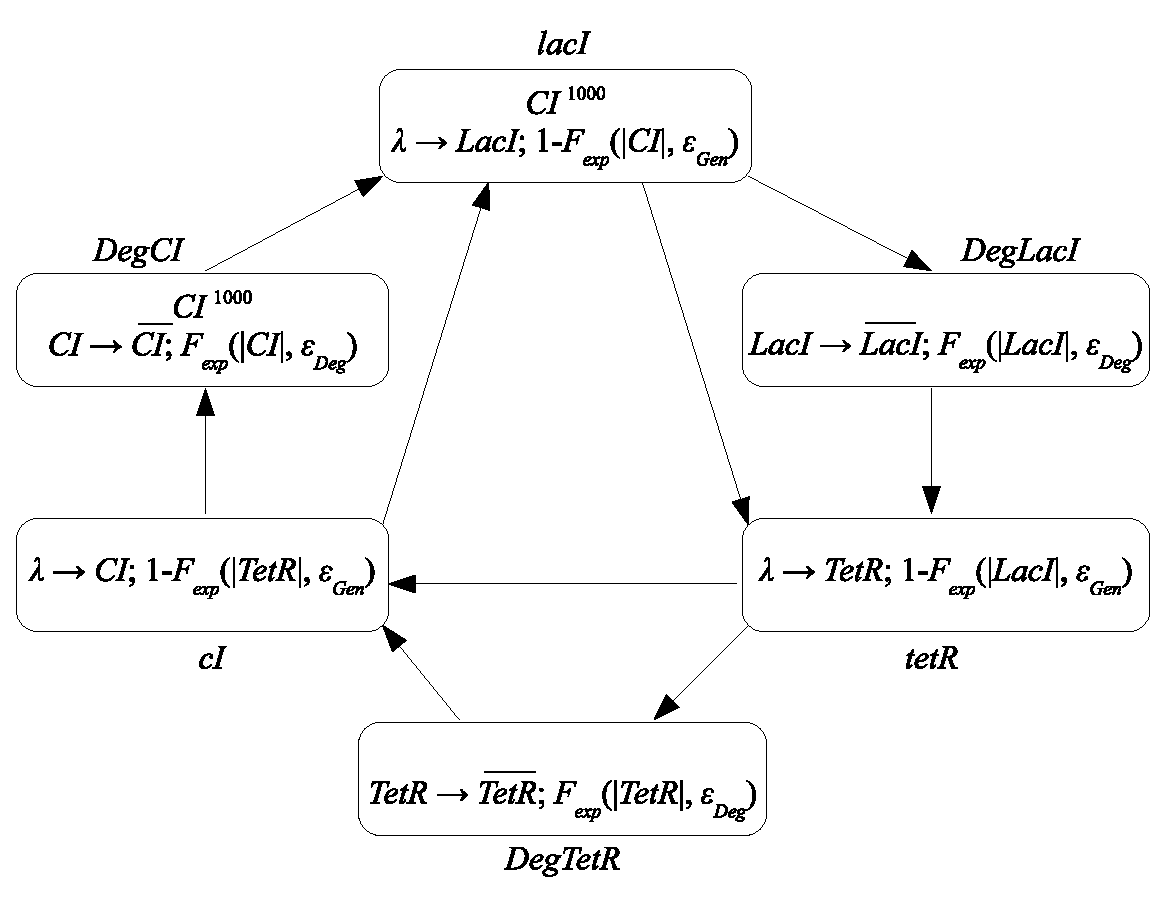
\includegraphics[width=0.67\textwidth]{DiagRepress}
\caption{The \textit{repressilator} model using BP system. Each of the three genes has an inhibitory effect on the next gene in the cycle. This is modelled by means of probability functions of the form $1-F_{exp}(..,..)$, which decreases the likelihood of the synthesis rule executing, the more inhibitor protein is present.}
\label{f:DiagRepress}
\end{center}
\end{figure}

The system is composed of three synthesis regions ---\textit{lacI}, \textit{tetR} and \textit{cI}--- connected with each other to form a ring, and their respective degradation regions ---\textit{DegLacI}, \textit{DegTetR} and \textit{DegCI}. The synthesis regions propagate copies of proteins by means of rules of the form $\lambda \rightarrow p_i; F_\sigma$, where $F_\sigma=1-F_{exp}(|p_j|, \epsilon_{Gen})$. Accordingly, as each gene has an inhibitory effect on the next one in the cycle, the more copies of the inhibitor protein $ p_j$ there are, the less likely the rule is to execute and therefore generate a copy of $p_i$. The degradation regions propagate anti-proteins of $p_i$ with a probability of $F_{exp}(|p_i|, \epsilon_{Deg} )$. The stability of the oscillations, the period of oscillation and the number of copies of each protein generated in each cycle can be controlled by the choice of parameters $\epsilon_{Gen}$ and $\epsilon_{Deg}$.

The model simulation shows that the system exhibits a stable and continuous oscillation, where all three genes, \textit{lacI}, \textit{tetR} and \textit{cI}, are activated one after the other in the order in which they appear in the cycle. Fig.~\ref{f:repress} shows the evolution of the number of copies of the proteins present in the system in two different simulations with parameters $\epsilon_{Gen} = 0.1$ and $\epsilon_{Deg} = 0.00125$ (Fig.~\ref{f:repress}a) and $\epsilon_{Gen} = 33.33$ and $\epsilon_{Deg} = 0.2$ (Fig.~\ref{f:repress}b). In the first case, we find that the oscillations are slow and the cycles long, but a lot of proteins are generated. In the second case, on the other hand, the oscillations are very fast (short cycles), but few proteins are generated. The two simulations differ as to how sensitive the regions are to the presence of proteins: they are less sensitive with $\epsilon_{Gen} = 0.1$ and $\epsilon_{Deg} = 0.00125$ (Fig.~\ref{f:repress}a) than with $\epsilon_{Gen} = 33.33$ and $\epsilon_{Deg} = 0.2$ (Fig.~\ref{f:repress}b), meaning that both synthesis and degradation are very slow, leading to longer oscillation cycles

\begin{figure}
\begin{center}
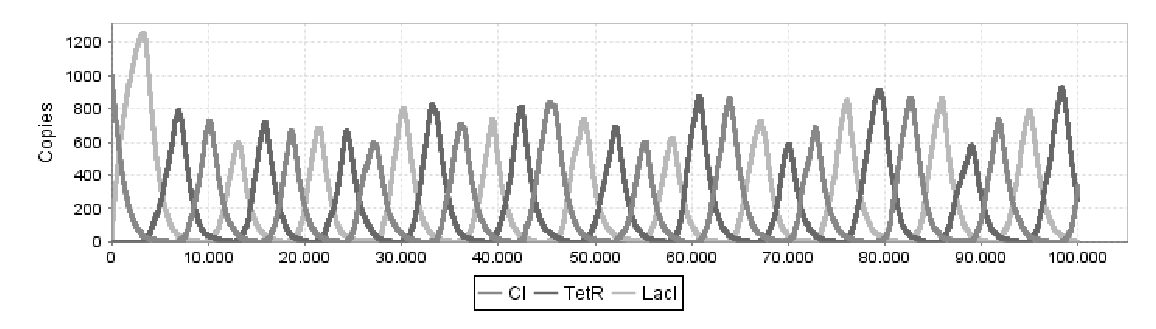
\includegraphics[width=1\textwidth]{repress1}
(a)
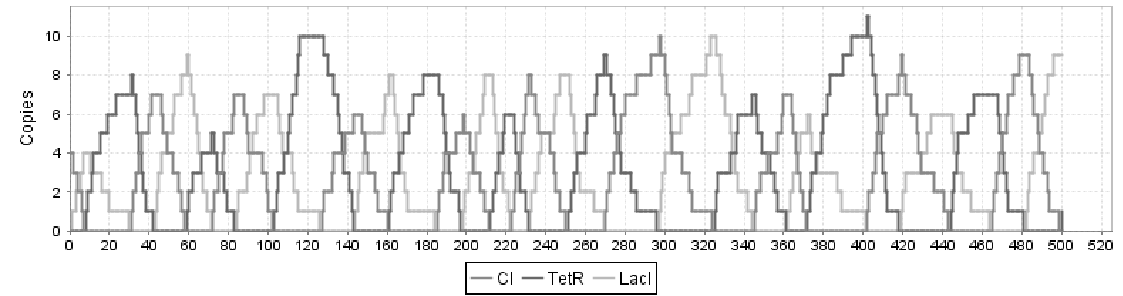
\includegraphics[width=1\textwidth]{repress2}
(b)
\caption{Two simulations of the \textit{repressilator} with parameters $\epsilon_{Gen} = 0.1$ and $\epsilon_{Deg} = 0.00125$ (a) and $\epsilon_{Gen} = 33.33$ and $\epsilon_{Deg} = 0.2$ (b). Small values of $\epsilon_{Gen}$ and $\epsilon_{Deg}$ (a) lead to long cycles generating a large quantity of proteins, whereas large values (b) make the system oscillate much faster generating fewer proteins.}
\label{f:repress}
\end{center}
\end{figure}

\begin{figure}
\begin{center}
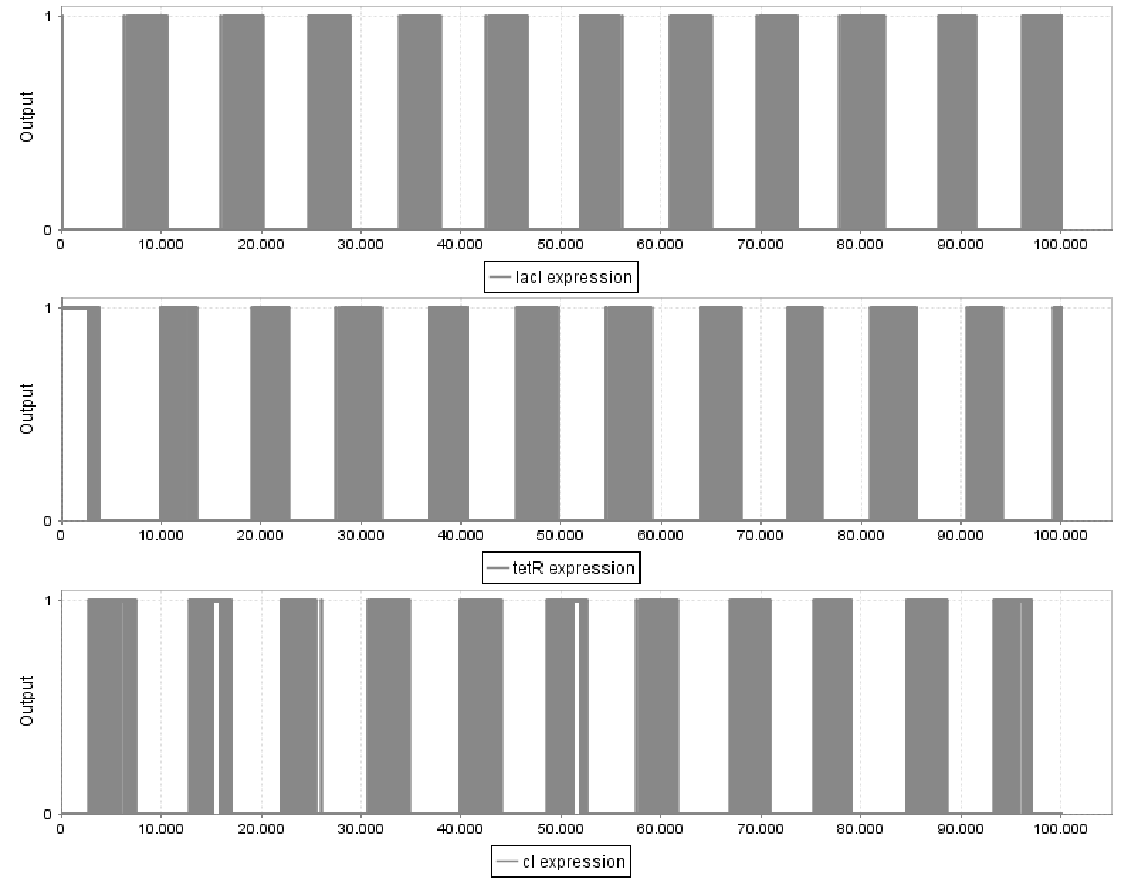
\includegraphics[width=1\textwidth]{sim}
\caption{Gene expression in the simulation with parameters $\epsilon_{Gen} = 0.1$ and $\epsilon_{Deg} = 0.00125$. There are successive periods of gene expression in the order in which the genes appear in the network, and the periods of expression are of similar duration and overlap with approximately the last third of the previous gene.}
\label{f:sim2}
\end{center}
\end{figure}

Fig.~\ref{f:sim2} also shows the system oscillation in the period of gene expression for the case of $\epsilon_{Gen} = 0.1$ and $\epsilon_{Deg} = 0.00125$: Genes exhibit very long periods of expression, of the order of 4000 simulation iterations, where iterations in which the synthesis rule is and is not executed alternate in frequent transitions from 0 to 1 and vice versa. Because of the transition frequency, the periods of expression are displayed as solid bars in the chart. Upon closer observation (see Fig.~\ref{f:detail}), however, it is apparent how the period of expression starts and ends gradually with sporadic protein propagations that steadily increase in frequency until they succeed each other continuously from iterations 81000 to 81750. They then slow down until they come to a complete standstill, and subsequently start up again in the next period of activity. In other words, when the expression intensity of one gene drops, the next gene starts to exhibit activity so that one gene is always being expressed.

\begin{figure}
\begin{center}
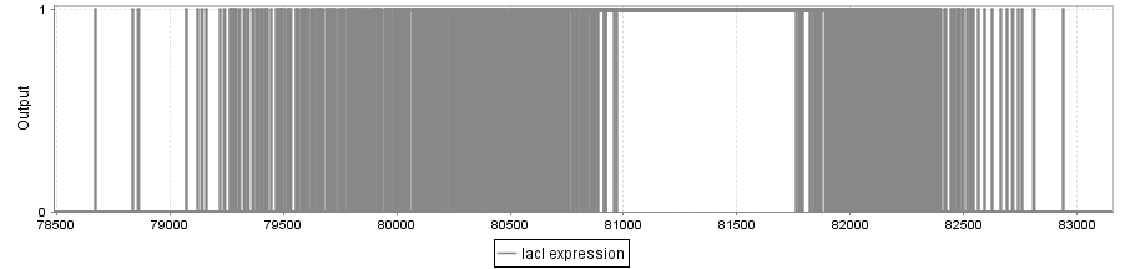
\includegraphics[width=1\textwidth]{detail}
\caption{Detail of the expression of \textit{lacI} in the simulation with parameters $\epsilon_{Gen} = 0.1$ and $\epsilon_{Deg} = 0.00125$ from iterations 78500 to 83000. As the inhibitory proteins \textit{CI} decrease (are degraded), the gene starts to be expressed, first sporadically and then gradually more and more often, stabilizing at 1 until approximately iteration 81750. At this point, copies of \textit{CI} arrive again and gradually start to inhibit gene expression.}
\label{f:detail}
\end{center}
\end{figure}
%
\section{Conclusions}
Bursting P systems are a feasible and realistic way of building qualitative models of genetic regulatory networks, as demonstrated by the \textit{repressilator} example presented as case study. These systems emulate the mechanism producing protein bursts in biological cells, using rules that are executed probabilistically depending on the number of copies of the regulatory proteins. Gene response to the presence of transcription factors is modelled by means of exponential probability distributions whose parameter regulates their sensitivity to the presence of copies of activator/inhibitor proteins. On the other hand, these same probability distributions are also used to model the exponential decay of the degrading proteins. In sum, the use of probability distributions enables the model to account for randomness, stochasticity, noise and fuzzy behaviour, as would be expected of a real system.


Although we have used exponential probability functions in this paper, it might be worthwhile to research the behaviour of these systems using other distribution functions in the future. Additionally, the model only accounts for the effect of transcription factors on the frequency of the bursts, all of which are of the same size, as the execution of a rule produces a single copy of a protein object. But, as suggested in~\cite{Raj2006}, it is conceivable that the presence of transcription factors might influence the amplitude (that is, the size) of those bursts rather than their frequency. Thus, it might be worthwhile examining how the system would work with rules like $\lambda \rightarrow p^r$, with $r \geq1$, where the number $r$ of copies of the protein $p$ produced would somehow, either deterministically or stochastically, be a function of the number of transcription factors. 

\bibliography{paper}{}
\bibliographystyle{plain}

\end{document}

